\documentclass{beamer}\usepackage[]{graphicx}\usepackage[]{color}
% maxwidth is the original width if it is less than linewidth
% otherwise use linewidth (to make sure the graphics do not exceed the margin)
\makeatletter
\def\maxwidth{ %
  \ifdim\Gin@nat@width>\linewidth
    \linewidth
  \else
    \Gin@nat@width
  \fi
}
\makeatother

\definecolor{fgcolor}{rgb}{0.345, 0.345, 0.345}
\newcommand{\hlnum}[1]{\textcolor[rgb]{0.686,0.059,0.569}{#1}}%
\newcommand{\hlstr}[1]{\textcolor[rgb]{0.192,0.494,0.8}{#1}}%
\newcommand{\hlcom}[1]{\textcolor[rgb]{0.678,0.584,0.686}{\textit{#1}}}%
\newcommand{\hlopt}[1]{\textcolor[rgb]{0,0,0}{#1}}%
\newcommand{\hlstd}[1]{\textcolor[rgb]{0.345,0.345,0.345}{#1}}%
\newcommand{\hlkwa}[1]{\textcolor[rgb]{0.161,0.373,0.58}{\textbf{#1}}}%
\newcommand{\hlkwb}[1]{\textcolor[rgb]{0.69,0.353,0.396}{#1}}%
\newcommand{\hlkwc}[1]{\textcolor[rgb]{0.333,0.667,0.333}{#1}}%
\newcommand{\hlkwd}[1]{\textcolor[rgb]{0.737,0.353,0.396}{\textbf{#1}}}%
\let\hlipl\hlkwb

\usepackage{framed}
\makeatletter
\newenvironment{kframe}{%
 \def\at@end@of@kframe{}%
 \ifinner\ifhmode%
  \def\at@end@of@kframe{\end{minipage}}%
  \begin{minipage}{\columnwidth}%
 \fi\fi%
 \def\FrameCommand##1{\hskip\@totalleftmargin \hskip-\fboxsep
 \colorbox{shadecolor}{##1}\hskip-\fboxsep
     % There is no \\@totalrightmargin, so:
     \hskip-\linewidth \hskip-\@totalleftmargin \hskip\columnwidth}%
 \MakeFramed {\advance\hsize-\width
   \@totalleftmargin\z@ \linewidth\hsize
   \@setminipage}}%
 {\par\unskip\endMakeFramed%
 \at@end@of@kframe}
\makeatother

\definecolor{shadecolor}{rgb}{.97, .97, .97}
\definecolor{messagecolor}{rgb}{0, 0, 0}
\definecolor{warningcolor}{rgb}{1, 0, 1}
\definecolor{errorcolor}{rgb}{1, 0, 0}
\newenvironment{knitrout}{}{} % an empty environment to be redefined in TeX

\usepackage{alltt}
\usetheme{Boadilla}

\makeatother
\setbeamertemplate{footline}
{
    \leavevmode%
    \hbox{%
    \begin{beamercolorbox}[wd=.4\paperwidth,ht=2.25ex,dp=1ex,center]{author in head/foot}%
        \usebeamerfont{author in head/foot}\insertshortauthor
    \end{beamercolorbox}%
    \begin{beamercolorbox}[wd=.55\paperwidth,ht=2.25ex,dp=1ex,center]{title in head/foot}%
        \usebeamerfont{title in head/foot}\insertshorttitle
    \end{beamercolorbox}%
    \begin{beamercolorbox}[wd=.05\paperwidth,ht=2.25ex,dp=1ex,center]{date in head/foot}%
        \insertframenumber{}
    \end{beamercolorbox}}%
    \vskip0pt%
}
\makeatletter
\setbeamertemplate{navigation symbols}{}

\usepackage[T1]{fontenc}
\usepackage{lmodern}
\usepackage{amssymb,amsmath,bm,bbm}
\renewcommand{\familydefault}{\sfdefault}

\DeclareMathOperator*{\argmax}{argmax}

\usepackage{mathtools}
\usepackage{graphicx}
\usepackage{threeparttable}
\usepackage{booktabs}
\usepackage{siunitx}
\sisetup{parse-numbers=false}

\setlength{\OuterFrameSep}{-2pt}
\makeatletter
\preto{\@verbatim}{\topsep=-10pt \partopsep=-10pt }
\makeatother

\title[Week 6:\ Maximum Likelihood Estimation]{Week 6:\ Maximum Likelihood Estimation}
\author[ResEcon 703:\ Advanced Econometrics]{ResEcon 703:\ Topics in Advanced Econometrics}
\date{Matt Woerman\\University of Massachusetts Amherst}
\IfFileExists{upquote.sty}{\usepackage{upquote}}{}
\begin{document}


{\setbeamertemplate{footline}{} 
\begin{frame}[noframenumbering]
    \titlepage
\end{frame}
}

\begin{frame}\frametitle{Agenda}
    Last two weeks
    \begin{itemize}
        \item Logit model
    \end{itemize}
    \vspace{3ex}
    This week's topics
    \begin{columns}
        \begin{column}{0.5\textwidth}
            \begin{itemize}
                \item \hyperlink{page.\getpagerefnumber{overview}}{Maximum likelihood overview}
                \item \hyperlink{page.\getpagerefnumber{estimator}}{Maximum likelihood estimator}
                \item \hyperlink{page.\getpagerefnumber{examples}}{Maximum likelihood examples}
                \item \hyperlink{page.\getpagerefnumber{properties}}{Properties of the maximum likelihood estimator}
            \end{itemize}
            \vspace{\fill}
        \end{column}
        \begin{column}{0.5\textwidth}
            \begin{itemize}
                \item \hyperlink{page.\getpagerefnumber{variance}}{MLE variance estimator}
                \item \hyperlink{page.\getpagerefnumber{fit}}{Model fit and tests}
                \item \hyperlink{page.\getpagerefnumber{optim}}{Numerical optimization}
                \item \hyperlink{page.\getpagerefnumber{example}}{Maximum likelihood estimation R example}
            \end{itemize}
        \end{column}
    \end{columns}
    \vspace{3ex}
    This week's reading
    \begin{itemize}
        \item Maximum likelihood estimation supplement
        \item Train textbook, chapter 8
    \end{itemize}
\end{frame}

\section{Maximum Likelihood Overview}
\label{overview}
\begin{frame}\frametitle{}
    \vfill
    \centering
    \begin{beamercolorbox}[center]{title}
        \Large Maximum Likelihood Overview
    \end{beamercolorbox}
    \vfill
\end{frame}

\begin{frame}\frametitle{Recap and Looking Ahead}
    Last three weeks
    \begin{itemize}
        \item Discrete choice framework
        \item Random utility model
        \item Logit model
    \end{itemize}
    \vspace{3ex}
    But we still do not know how to estimate the logit model! \\
    \vspace{3ex}
    Next two weeks
    \begin{itemize}
        \item Maximum likelihood estimation
        \item Numerical optimization
        \item Estimating the logit model
    \end{itemize}
\end{frame}

\begin{frame}\frametitle{Maximum Likelihood Estimation}
    Maximum likelihood (ML) estimation is one of the most common estimation methods in structural econometrics
    \begin{itemize}
        \item ML is more flexible than OLS regression
        \begin{itemize}
            \item ML can accommodate nonlinear models
            \item OLS is a special case of ML
        \end{itemize}
        \item ML requires stronger distributional assumptions than OLS
        \begin{itemize}
            \item When these assumptions hold, the maximum likelihood estimator (MLE) is consistent and efficient
            \item But if these assumptions are invalid, the interpretation is less clear
        \end{itemize}
    \end{itemize}
    \vspace{3ex}
    Overview of maximum likelihood estimation
    \begin{itemize}
        \item ML requires distributional assumptions about the data-generating process you observe
        \item MLE are the parameters that make it most likely to generate the observed data
    \end{itemize}
\end{frame}

\begin{frame}\frametitle{Maximum Likelihood Intuition}
    Suppose we have five random draws from a normal distribution, but we do not know which normal distribution, $\mathcal{N}(\mu, \sigma^2)$
    $$\bm{y} = \{48.7, 50.9, 48.8, 50.6, 48.8\}$$
    Consider two candidate distributions
    $$\mathcal{N}(0, 1) \quad \text{or} \quad \mathcal{N}(50, 1)$$ \\
    \begin{itemize}
        \item What is the likelihood of generating $\bm{y}$ from $\mathcal{N}(0, 1)$?
        \begin{itemize}
            \item Practically zero
        \end{itemize}
        \item What is the likelihood of generating $\bm{y}$ from $\mathcal{N}(50, 1)$?
        \begin{itemize}
            \item Much greater!
        \end{itemize}
        \item Given these data, $\bm{y}$, $\mu = 50$ has a greater likelihood than $\mu = 0$
    \end{itemize}
    \vspace{2ex}
    This is a simple example of the intuition of maximum likelihood estimation
    \begin{itemize}
        \item Find the parameters that maximize the likelihood of generating the data you observe
    \end{itemize}
\end{frame}

\begin{frame}\frametitle{Probability Density Function}
    The probability density function, $f(y \mid \bm{\theta})$, gives us the relative likelihood that a random variable would take a particular value \\
    \vspace{2ex}
    The probability density function of the normal distribution is
    $$f(y \mid \mu, \sigma^2) = \frac{1}{\sqrt{2 \pi \sigma^2}} e^{\frac{-(y - \mu)^2}{2 \sigma^2}}$$ \\
    \begin{center}
        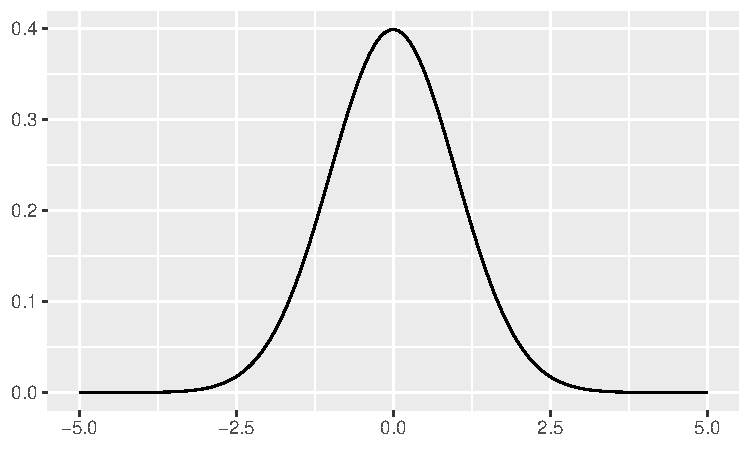
\includegraphics[width=0.6\textwidth]{norm_pdf.pdf}
    \end{center}
    \vspace{-2ex}
\end{frame}

\begin{frame}\frametitle{Likelihood}
    But what if the opposite is true---we know the outcome of the random variable draw, but we do not know the parameters that generated it?
    \begin{itemize}
        \item We can use the same mathematical expression to give us the likelihood that a particular set of parameter values would have generated that sample
        \item We call this the likelihood function and denote it as $L(\bm{\theta} \mid \bm{y})$
    \end{itemize}
    \vspace{2ex}
    The likelihood function for a single known random draw, $y$, from the normal distribution is
    $$L(\mu, \sigma^2 \mid y) = \frac{1}{\sqrt{2 \pi \sigma^2}} e^{\frac{-(y - \mu)^2}{2 \sigma^2}}$$
\end{frame}

\section{Maximum Likelihood Estimator}
\label{estimator}
\begin{frame}\frametitle{}
    \vfill
    \centering
    \begin{beamercolorbox}[center]{title}
        \Large Maximum Likelihood Estimator
    \end{beamercolorbox}
    \vfill
\end{frame}

\begin{frame}\frametitle{Maximum Likelihood Estimation Assumption}
    The probability density function for a random variable, $y$, conditioned on a set of parameters, $\bm{\theta}$, is
    $$f(y \mid \bm{\theta})$$ \\
    \begin{itemize}
        \item This function identifies the data-generating process that underlies an observed sample of data and provides a mathematical description of the data that the process will produce
        \item We are making an assumption about the density of $y$, not just its expectation and variance
    \end{itemize}
    \vspace{3ex}
    We could generalize to a random vector, $\bm{y}$, with joint density $f(\bm{y} \mid \bm{\theta})$
    \begin{itemize}
        \item But the random variable assumption will be sufficient for this course
    \end{itemize}
\end{frame}

\begin{frame}\frametitle{Likelihood Function}
    The joint density of $n$ independent and identically distributed (i.i.d.) random variables, each with density $f(y \mid \bm{\theta})$, is
    $$f(y_1, \ldots, y_n \mid \bm{\theta}) = \prod_{i = 1}^n f(y_i \mid \bm{\theta})$$ \\
    \vspace{2ex}
    This representation suggests that the parameters are known and the data are unknown, but usually the opposite is true
    \begin{itemize}
        \item We have data and want to know the parameters of the data-generating process
    \end{itemize}
    \vspace{2ex}
    We simply switch the conditioning and define the likelihood function as a function of the unknown parameters, $\bm{\theta}$, conditioned on the data we observe, $\bm{y}$
    $$L(\bm{\theta} \mid \bm{y}) = \prod_{i = 1}^n f(y_i \mid \bm{\theta})$$
\end{frame}

\begin{frame}\frametitle{Log-Likelihood Function}
    The likelihood function of unknown parameters $\bm{\theta}$ conditioned on the data $\bm{y}$ is
    $$L(\bm{\theta} \mid \bm{y}) = \prod_{i = 1}^n f(y_i \mid \bm{\theta})$$ \\
    \vspace{2ex}
    It is usually easier to work with the log of this likelihood function, or the log-likelihood function, so we have a sum instead of a product on the right-hand side
    $$\ln L(\bm{\theta} \mid \bm{y}) = \sum_{i = 1}^n \ln f(y_i \mid \bm{\theta})$$ \\
    \vspace{2ex}
    Log is a monotonic transformation, so finding the greatest log-likelihood will get us the same result as finding the greatest likelihood
\end{frame}

\begin{frame}\frametitle{Maximum Likelihood Estimator}
    The maximum likelihood estimator, $\widehat{\bm{\theta}}$, is the set of parameters that maximizes the likelihood function and log-likelihood function
    \begin{align*}
        \widehat{\bm{\theta}} & = \argmax_{\bm{\theta}} L(\bm{\theta} \mid \bm{y}) \\
        \widehat{\bm{\theta}} & = \argmax_{\bm{\theta}} \ln L(\bm{\theta} \mid \bm{y})
    \end{align*} \\
    \vspace{2ex}
    A necessary condition for maximizing $\ln L(\bm{\theta} \mid \bm{y})$ is
    $$\frac{\partial \ln L(\bm{\theta} \mid \bm{y})}{\partial \bm{\theta}} = \bm{0}$$ \\
    \vspace{2ex}
    The maximum likelihood estimator gives the parameter values that maximize the likelihood of having generated the data that we observe
\end{frame}

\begin{frame}\frametitle{Conditional Likelihood}
    So far, we have assumed our data, $\bm{y}$, are conditional on only parameters
    \begin{itemize}
        \item But we usually model our outcome data, $\bm{y}$, as a function of both parameters, $\bm{\theta}$, and other data, $\bm{X}$
    \end{itemize}
    \vspace{2ex}
    When $y$ is also a function of $\bm{x}$, we need to define its conditional probability density function, $f(y \mid \bm{x}, \bm{\theta})$ \\
    \vspace{2ex}
    In almost all cases, we can simply use $f(y \mid \bm{x}, \bm{\theta})$ in place of $f(y \mid \bm{\theta})$ in the definition of the likelihood function and log-likelihood function
    \vspace{-1ex}
    \begin{align*}
        L(\bm{\theta} \mid \bm{y}, \bm{X}) & = \prod_{i = 1}^n f(y_i \mid \bm{x}_i, \bm{\theta}) \\
        \ln L(\bm{\theta} \mid \bm{y}, \bm{X}) & = \sum_{i = 1}^n \ln f(y_i \mid \bm{x}_i, \bm{\theta})
    \end{align*} \\
    \vspace{-1ex}
    \begin{itemize}
        \item This is technically a conditional likelihood function, but we often drop the ``conditional'' for convenience
    \end{itemize}
\end{frame}

\section{Maximum Likelihood Examples}
\label{examples}
\begin{frame}\frametitle{}
    \vfill
    \centering
    \begin{beamercolorbox}[center]{title}
        \Large Maximum Likelihood Examples
    \end{beamercolorbox}
    \vfill
\end{frame}

\begin{frame}\frametitle{Maximum Likelihood Poisson Example}
    We have ten data points from a Poisson distribution, but what is the $\lambda$ parameter of the distribution?
    $$\bm{y} = \{ 2, 0, 1, 2, 2, 2, 0, 2, 1, 1 \}$$ \\
    \vspace{-1ex}
    $$f(y \mid \lambda) = \frac{e^{-\lambda} \lambda^y }{y!}$$ \\
    \vspace{1ex}
    \begin{columns}
        \begin{column}{0.33\textwidth}
            $$f(y \mid \lambda = 1)$$ \\
            \vspace{-2ex}
            \begin{center}
                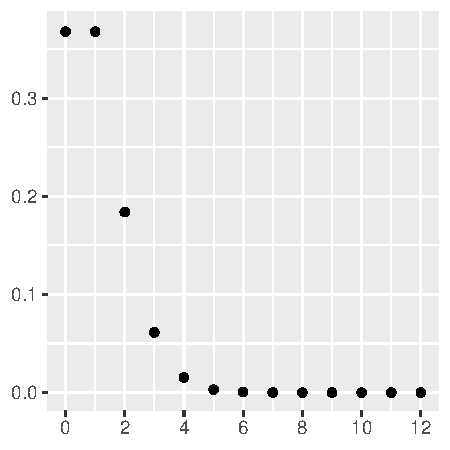
\includegraphics[width=0.9\textwidth]{pois_1_pmf.pdf}
            \end{center}
        \end{column}
        \begin{column}{0.33\textwidth}
            $$f(y \mid \lambda = 3)$$ \\
            \vspace{-2ex}
            \begin{center}
                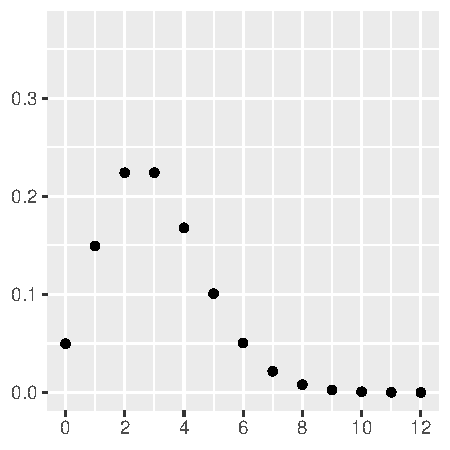
\includegraphics[width=0.9\textwidth]{pois_3_pmf.pdf}
            \end{center}
        \end{column}
        \begin{column}{0.33\textwidth}
            $$f(y \mid \lambda = 5)$$ \\
            \vspace{-2ex}
            \begin{center}
                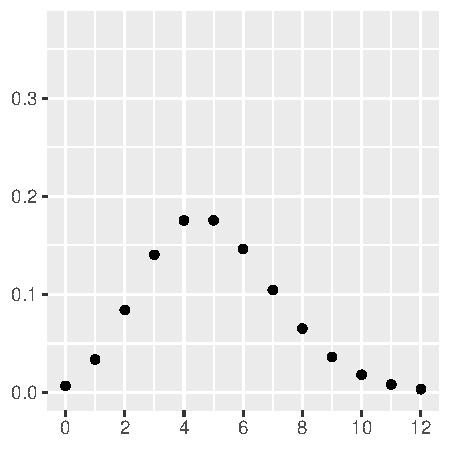
\includegraphics[width=0.9\textwidth]{pois_5_pmf.pdf}
            \end{center}
        \end{column}
    \end{columns}
\end{frame}

\begin{frame}\frametitle{Maximum Likelihood Poisson Example}
    We have ten data points from a Poisson distribution, but what is the $\lambda$ parameter of the distribution?
    $$\bm{y} = \{ 2, 0, 1, 2, 2, 2, 0, 2, 1, 1 \}$$
    \begin{align*}
        L(\lambda \mid \bm{y}) & = \prod_{i = 1}^n \frac{e^{-\lambda} \lambda^{y_i} }{y_i!} = \frac{e^{-n \lambda} \lambda^{\sum_{i=1}^n y_i}}{\prod_{i = 1}^n y_i!} \\
        \ln L(\lambda \mid \bm{y}) & = -n \lambda + \ln \lambda \sum_{i = 1}^n y_i - \sum_{i = 1}^n \ln (y_i!) \\
        \frac{\partial \ln L(\lambda \mid \bm{y})}{\partial \lambda} & = -n + \frac{1}{\lambda} \sum_{i = 1}^n y_i \\
        \frac{\partial \ln L(\lambda \mid \bm{y})}{\partial \lambda} & = 0 ~~ \Rightarrow ~~ \widehat{\lambda} = \frac{1}{n} \sum_{i = 1}^n y_i = 1.3
    \end{align*}
\end{frame}

\begin{frame}\frametitle{Maximum Likelihood Poisson Example}
    We have ten data points from a Poisson distribution, but what is the $\lambda$ parameter of the distribution?
    $$\bm{y} = \{ 2, 0, 1, 2, 2, 2, 0, 2, 1, 1 \}$$
    \begin{align*}
        L(\lambda \mid \bm{y}) & = \prod_{i = 1}^n \frac{e^{-\lambda} \lambda^{y_i} }{y_i!} = \frac{e^{-n \lambda} \lambda^{\sum_{i=1}^n y_i}}{\prod_{i = 1}^n y_i!} = \frac{e^{-10 \lambda} \lambda^{\sum_{i=1}^n 13}}{32}\\
        \ln L(\lambda \mid \bm{y}) & = -n \lambda + \ln \lambda \sum_{i = 1}^n y_i - \sum_{i = 1}^n \ln (y_i!) = -10 \lambda + 13 \ln \lambda - 3.47\\
    \end{align*} \\
    \vspace{-4ex}
    \begin{center}
        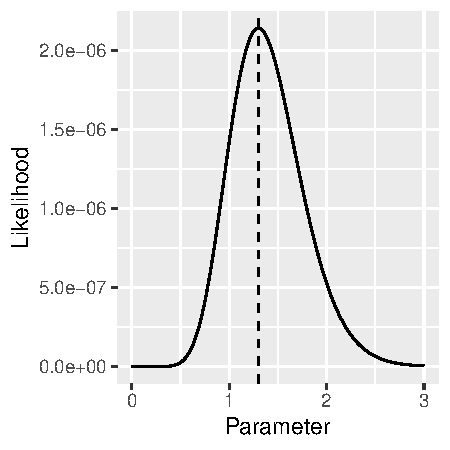
\includegraphics[width=0.26\textwidth]{likelihood.pdf}
        \hspace{5ex}
        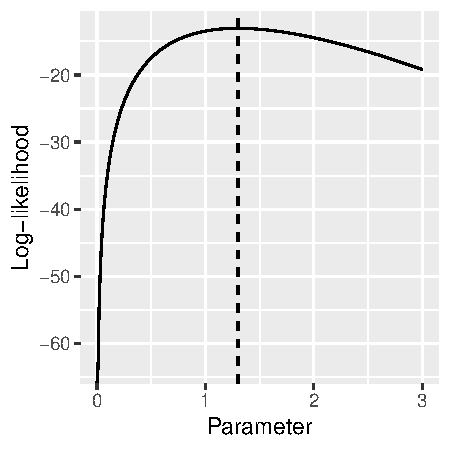
\includegraphics[width=0.26\textwidth]{log_likelihood.pdf}
    \end{center}
\end{frame}

\begin{frame}\frametitle{Maximum Likelihood Normal Example}
    We have five data points from a normal distribution, but what are the $\mu$ and $\sigma^2$ parameters of the distribution?
    $$\bm{y} = \{ 6.08, 5.29, 2.52, 2.94, 5.36 \}$$ \\
    \vspace{-3ex}
    \begin{align*}
        f(y \mid \mu, \sigma^2) & = \frac{1}{\sqrt{2 \pi \sigma^2}} e^{\frac{-(y - \mu)^2}{2 \sigma^2}} \\
        L(\mu, \sigma^2 \mid \bm{y}) & = \left( \frac{1}{\sqrt{2 \pi \sigma^2}} \right)^n e^{-\frac{1}{2 \sigma^2} \sum_{i = 1}^n (y_i - \mu)^2} \\
        \ln L(\mu, \sigma^2 \mid \bm{y}) & = -\frac{n}{2} \ln 2 \pi - \frac{n}{2} \ln \sigma^2 - \frac{1}{2 \sigma^2} \sum_{i = 1}^n (y_i - \mu)^2 \\
        \frac{\partial \ln L(\mu, \sigma^2 \mid \bm{y})}{\partial \mu} & = \frac{1}{\sigma^2} \sum_{i = 1}^n (y_i - \mu) \\
        \frac{\partial \ln L(\mu, \sigma^2 \mid \bm{y})}{\partial \sigma^2} & = - \frac{n}{2 \sigma^2} + \frac{1}{2 \sigma^4} \sum_{i = 1}^n (y_i - \mu)^2
    \end{align*} \\
    \vspace{-2ex}
\end{frame}

\begin{frame}\frametitle{Maximum Likelihood Normal Example}
    We have five data points from a normal distribution, but what are the $\mu$ and $\sigma^2$ parameters of the distribution?
    $$\bm{y} = \{ 6.08, 5.29, 2.52, 2.94, 5.36 \}$$
    \begin{align*}
        \frac{\partial \ln L(\mu, \sigma^2 \mid \bm{y})}{\partial \mu} & = \frac{1}{\sigma^2} \sum_{i = 1}^n (y_i - \mu) \\
        \frac{\partial \ln L(\mu, \sigma^2 \mid \bm{y})}{\partial \sigma^2} & = - \frac{n}{2 \sigma^2} + \frac{1}{2 \sigma^4} \sum_{i = 1}^n (y_i - \mu)^2
    \end{align*}
    \begin{align*}
        \frac{\partial \ln L(\mu, \sigma^2 \mid \bm{y})}{\partial \mu} & = 0 ~~ \Rightarrow ~~ \widehat{\mu} = \frac{1}{n} \sum_{i = 1}^n y_i = 4.44 \\
        \frac{\partial \ln L(\mu, \sigma^2 \mid \bm{y})}{\partial \sigma^2} & = 0 ~~ \Rightarrow ~~ \widehat{\sigma}^2 = \frac{1}{n} \sum_{i = 1}^n (y_i - \widehat{\mu})^2 = 2.04
    \end{align*} \\
    \vspace{-2ex}
\end{frame}

\begin{frame}\frametitle{Maximum Likelihood OLS Regression Example}
    In the previous two examples, we have estimated the parameters that maximize the likelihood of generating the data that we observe \\
    \vspace{2ex}
    But in most econometric applications, we really want to estimate the parameters that maximize the likelihood of generating our outcome data (or dependent variable) conditional on the other data (or independent variables) that we observe
    \begin{itemize}
        \item A basic example is a simple OLS regression
    \end{itemize}
    $$y_i = \beta_0 + \beta_1 x_i + \varepsilon_i$$ \\
    \vspace{2ex}
    If we make a distributional assumption about $\varepsilon_i$, then we can estimate the parameters of this model using maximum likelihood
    $$\varepsilon_i \sim \mathcal{N}(0, \sigma^2)$$
\end{frame}

\begin{frame}\frametitle{Maximum Likelihood OLS Regression Example}
    Combining our simple OLS regression equation
    \begin{align*}
        y_i & = \beta_0 + \beta_1 x_i + \varepsilon_i
        \intertext{with the distributional assumption about the error term}
        \varepsilon_i & \sim \mathcal{N}(0, \sigma^2)
        \intertext{gives us a conditional distribution of $y_i$}
        y_i \mid x_i & \sim \mathcal{N}(\beta_0 + \beta_1 x_i, \sigma^2)
    \end{align*} \\
    \vspace{2ex}
    Then the conditional probability density function of $y_i$ is
    $$f(y_i \mid x_i, \beta_0, \beta_1, \sigma^2) = \frac{1}{\sqrt{2 \pi \sigma^2}} e^{\frac{-(y_i - \beta_0 - \beta_1 x_i)^2}{2 \sigma^2}}$$
\end{frame}

\begin{frame}\frametitle{Maximum Likelihood OLS Regression Example}
    The (conditional) log-likelihood function is
    $$\ln L(\beta_0, \beta_1, \sigma^2 \mid \bm{y}, \bm{x}) = -\frac{n}{2} \ln 2 \pi - \frac{n}{2} \ln \sigma^2 - \frac{1}{2 \sigma^2} \sum_{i = 1}^n (y_i - \beta_0 - \beta_1 x_i)^2$$ \\
    \vspace{2ex}
    Taking the derivative with respect to each parameter---$\beta_0$, $\beta_1$, and $\sigma^2$---and setting them equal to zero yields the OLS estimators
    \begin{align*}
        \widehat{\beta}_1 & = \frac{\sum_{i = 1}^n (x_i - \bar{x})(y_i - \bar{y})}{\sum_{i = 1}^n (x_i - \bar{x})^2} \\
        \widehat{\beta}_0 & = \bar{y} - \widehat{\beta}_1 \bar{x} \\
        \widehat{\sigma}^2 & = \frac{1}{n} \sum_{i = 1}^n (y_i - \widehat{\beta}_0 - \widehat{\beta}_1 x_i)^2
    \end{align*} \\
    \vspace{-2ex}
\end{frame}

\section{Properties of the Maximum Likelihood Estimator}
\label{properties}
\begin{frame}\frametitle{}
    \vfill
    \centering
    \begin{beamercolorbox}[center]{title}
        \Large Properties of the Maximum Likelihood Estimator
    \end{beamercolorbox}
    \vfill
\end{frame}

\begin{frame}\frametitle{Asymptotic Properties of MLE}
    Under certain regularity conditions, the maximum likelihood estimator (MLE) has these properties
    \begin{enumerate}
        \item Consistency
        \item Asymptotic normality
        \item Asymptotic efficiency
        \item Invariance
    \end{enumerate}
\end{frame}

\begin{frame}\frametitle{Regularity Conditions for MLE}
    The following properties are true only if these regularity conditions are met
    \begin{enumerate}
        \item The first three derivatives of $\ln f(y_i \mid \bm{\theta})$ with respect to $\bm{\theta}$ are continuous and finite for almost all $y_i$ and for all $\bm{\theta}$
        \item The conditions necessary to obtain the expectations of the first and second derivatives of $\ln f(y_i \mid \bm{\theta})$ are met
        \item For all values of $\bm{\theta}$, $\left\vert \frac{\partial^3 \ln f(y_i \mid \bm{\theta})}{\partial \theta_j \partial \theta_k \partial \theta_l} \right\vert$ is less than a function that has a
        finite expectation
    \end{enumerate}
\end{frame}

\begin{frame}\frametitle{Consistency of MLE}
    The MLE, $\widehat{\bm{\theta}}$, converges in probability to the true parameter value(s), $\bm{\theta}_0$
    $$\widehat{\bm{\theta}} \overset{p}{\rightarrow} \bm{\theta}_0$$ \\
    \begin{itemize}
        \item As our sample size grows (to infinity), the MLE becomes vanishingly close to the true parameter value(s)
    \end{itemize}
\end{frame}

\begin{frame}\frametitle{Asymptotic Normality of MLE}
    The asymptotic distribution of the MLE, $\widehat{\bm{\theta}}$, is normal with mean at the true parameter value(s), $\bm{\theta}_0$, and known variance
    $$\widehat{\bm{\theta}} \overset{a}{\sim} \mathcal{N} \left( \bm{\theta}_0, I(\bm{\theta}_0)^{-1} \right)$$
    where
    $$I(\bm{\theta}_0) = -E_0 \left[ \frac{\partial^2 \ln L(\bm{\theta}_0)}{\partial \bm{\theta}_0 \partial \bm{\theta}_0'} \right]$$
    \begin{itemize}
        \item The asymptotic variance-covariance matrix of the MLE is
        $$Var(\widehat{\bm{\theta}}) = \left\{ -E_0 \left[ \frac{\partial^2 \ln L(\bm{\theta}_0)}{\partial \bm{\theta}_0 \partial \bm{\theta}_0'} \right] \right\}^{-1}$$
        \item We are more certain of the MLE when the likelihood function has more curvature
    \end{itemize}
\end{frame}

\begin{frame}\frametitle{Asymptotic Efficiency of MLE}
    The MLE, $\widehat{\bm{\theta}}$, is asymptotically efficient and achieves the Cram\'er-Rao lower bound
    $$Var(\widehat{\bm{\theta}}) = I(\bm{\theta}_0)^{-1}$$
    \begin{itemize}
        \item No consistent estimator has lower asymptotic variance than the MLE
    \end{itemize}
\end{frame}

\begin{frame}\frametitle{Invariance of MLE}
    The MLE of $\bm{\gamma}_0 = \bm{c}(\bm{\theta}_0)$ is $\bm{c}(\widehat{\bm{\theta}})$ if $\bm{c}(\bm{\theta}_0)$ is continuous and continuously differentiable, where $\widehat{\bm{\theta}}$ is the MLE of true parameter(s) $\bm{\theta}_0$
    \begin{itemize}
        \item The MLE of a function of some parameter(s) is the function applied to the MLE of the parameter(s)
    \end{itemize}
\end{frame}

\section{MLE Variance Estimator}
\label{variance}
\begin{frame}\frametitle{}
    \vfill
    \centering
    \begin{beamercolorbox}[center]{title}
        \Large MLE Variance Estimator
    \end{beamercolorbox}
    \vfill
\end{frame}

\begin{frame}\frametitle{Variance of the Maximum Likelihood Estimator}
    From the asymptotic normality of MLE, the variance-covariance matrix of the MLE is
    $$Var(\widehat{\bm{\theta}}) = \left\{ -E_0 \left[ \frac{\partial^2 \ln L(\bm{\theta}_0)}{\partial \bm{\theta}_0 \partial \bm{\theta}_0'} \right] \right\}^{-1}$$
    \begin{itemize}
        \item The inner-most term (inside the $[~]$) is the Hessian of the log-likelihood function with respect to the parameters
        \item The term that is inverted (the $-E_0[~]$ term) is equivalent to the Fisher information matrix
        \item The variance of the MLE is evaluated at $\bm{\theta}_0$, the true parameter value(s), and requires taking an expectation
    \end{itemize}
\end{frame}

\begin{frame}\frametitle{Hessian of the Log-Likelihood Function}
    The Hessian of the log-likelihood function with respect to the parameters is the square matrix that contains the second derivative of the log-likelihood function with respect to all pairwise combinations of parameters
    $$\frac{\partial^2 \ln L(\bm{\theta}_0)}{\partial \bm{\theta}_0 \partial \bm{\theta}_0'} = \begin{pmatrix}
        \frac{\partial^2 \ln L(\bm{\theta}_0)}{\partial^2 \theta_1} & \frac{\partial^2 \ln L(\bm{\theta}_0)}{\partial \theta_1 \partial \theta_2} & \cdots & \frac{\partial^2 \ln L(\bm{\theta}_0)}{\partial \theta_1 \partial \theta_k} \\
        \frac{\partial^2 \ln L(\bm{\theta}_0)}{\partial \theta_1 \partial \theta_2} & \frac{\partial^2 \ln L(\bm{\theta}_0)}{\partial^2 \theta_2} & \cdots & \frac{\partial^2 \ln L(\bm{\theta}_0)}{\partial \theta_2 \partial \theta_k} \\
        \vdots & \vdots & \ddots & \vdots \\
        \frac{\partial^2 \ln L(\bm{\theta}_0)}{\partial \theta_1 \partial \theta_k} & \frac{\partial^2 \ln L(\bm{\theta}_0)}{\partial \theta_2 \partial \theta_k} & \cdots & \frac{\partial^2 \ln L(\bm{\theta}_0)}{\partial^2 \theta_k}
    \end{pmatrix}$$ \\
    \vspace{3ex}
    This matrix describes the local curvature of the log-likelihood function around the true parameter values, $\bm{\theta}_0$
\end{frame}

\begin{frame}\frametitle{Information Matrix Equality}
    The Fisher information matrix measures the amount of information that our data, $\bm{y}$ and $\bm{X}$, contains about the unknown parameters, $\bm{\theta}$
    $$I(\bm{\theta}_0) = E_0 \left[ \frac{\partial \ln L(\bm{\theta}_0)}{\partial \bm{\theta}_0} \frac{\partial \ln L(\bm{\theta}_0)}{\partial \bm{\theta}_0'} \right]$$ \\
    \vspace{3ex}
    The information matrix equality gives that the Fisher information matrix equals the negative of the expectation of the Hessian of the log-likelihood function
    $$E_0 \left[ \frac{\partial \ln L(\bm{\theta}_0)}{\partial \bm{\theta}_0} \frac{\partial \ln L(\bm{\theta}_0)}{\partial \bm{\theta}_0'} \right] = -E_0 \left[ \frac{\partial^2 \ln L(\bm{\theta}_0)}{\partial \bm{\theta}_0 \partial \bm{\theta}_0'} \right]$$
\end{frame}

\begin{frame}\frametitle{MLE Variance Estimator}
    The true variance-covariance matrix of the MLE is evaluated at the true parameter values, $\bm{\theta}$, and requires taking an expectation
    $$Var(\widehat{\bm{\theta}}) = \left\{ -E_0 \left[ \frac{\partial^2 \ln L(\bm{\theta}_0)}{\partial \bm{\theta}_0 \partial \bm{\theta}_0'} \right] \right\}^{-1}$$
    We can estimate this variance by evaluating the actual Hessian (not its expectation) at the MLE, $\widehat{\bm{\theta}}$ \\
    \vspace{2ex}
    The estimator of the MLE variance-covariance matrix is
    $$\widehat{Var}(\widehat{\bm{\theta}}) = \left\{ \left. -\frac{\partial^2 \ln L(\bm{\theta})}{\partial \bm{\theta} \partial \bm{\theta}'} \right\vert_{\bm{\theta} = \widehat{\bm{\theta}}} \right\}^{-1}$$ \\
    \vspace{2ex}
    More robust variance estimators exist, but we will use this most basic one
\end{frame}

\section{Model Fit and Tests}
\label{fit}
\begin{frame}\frametitle{}
    \vfill
    \centering
    \begin{beamercolorbox}[center]{title}
        \Large Model Fit and Tests
    \end{beamercolorbox}
    \vfill
\end{frame}

\begin{frame}\frametitle{Likelihood Ratio Index}
    One measure of how well a MLE fits the data is the likelihood ratio index
    $$\rho = 1 - \frac{\ln L(\widehat{\bm{\theta}})}{\ln L(\bm{0})}$$
    where $L(\bm{0})$ measures the fit of a model with only a constant term (all other parameters equal to 0)
    \begin{itemize}
        \item This index looks like $R^2$ and is sometimes called a ``pseudo $R^2$''
        \item But this name is misleading because this metric is nothing like $R^2$ other than having the same range of $[0, 1]$
    \end{itemize}
    \vspace{3ex}
    Larger values of $\rho$ imply a better model fit, but this is no different from saying larger values of the likelihood and log-likelihood functions are better
\end{frame}

\begin{frame}\frametitle{Hypothesis Tests}
    Suppose we want to test hypotheses about the parameters of our model
    $$H_0: \bm{h}(\bm{\theta}_0) = \bm{0}$$
    where $\bm{h}(\bm{\theta}_0)$ is any set of $J$ parameter restrictions \\
    \vspace{2ex}
    This specification of hypotheses is fully general
    \begin{itemize}
        \item We can test if parameters are equal to zero
        $$\bm{h}(\bm{\theta}_0) = \begin{pmatrix}
            \theta_1 \\
            \theta_2
        \end{pmatrix} = \begin{pmatrix}
            0 \\
            0
        \end{pmatrix}$$
        \item We can test if parameters are equal to each other
        $$\bm{h}(\bm{\theta}_0) = \begin{pmatrix}
            \theta_1 - \theta_3 \\
            \theta_2 - \theta_3
        \end{pmatrix} = \begin{pmatrix}
            0 \\
            0
        \end{pmatrix}$$
    \end{itemize}
\end{frame}

\begin{frame}\frametitle{Likelihood Ratio Test}
    The likelihood ratio test compares the log-likelihood values of the unrestricted model and the restricted model
    \begin{itemize}
        \item If the hypotheses are true, then these values should be close
    \end{itemize}
    \vspace{2ex}
    The likelihood ratio test statistic is 
    $$-2 \ln \lambda = 2 \left( \ln L(\widehat{\bm{\theta}}_U) - \ln L(\widehat{\bm{\theta}}_R) \right)$$ \\
    \vspace{-1ex}
    \begin{itemize}
        \item $\widehat{\bm{\theta}}_U$ is the MLE of the unrestricted model
        \item $\widehat{\bm{\theta}}_R$ is the MLE of the restricted model
        \item $\lambda$ is the likelihood ratio, $\lambda = L(\widehat{\bm{\theta}}_R) / L(\widehat{\bm{\theta}}_U)$ 
    \end{itemize}
    \vspace{2ex}
    This test statistic is distributed $\chi^2$ with degrees of freedom equal to the number of model restrictions
    $$-2 \ln \lambda \sim \chi^2(J)$$
\end{frame}

\begin{frame}\frametitle{Wald and Lagrange Multiplier Tests}
    Two other common tests for MLE parameters are the Wald test and the Lagrange multiplier test \\
    \vspace{2ex}
    Wald test
    \begin{itemize}
        \item If the hypotheses are true, then $\bm{h}(\widehat{\bm{\theta}}_U) \approx \bm{0}$
        \item Test if $\bm{h}(\widehat{\bm{\theta}}_U)$ is sufficiently close to $\bm{0}$
    \end{itemize}
    \vspace{2ex}
    Lagrange multiplier test
    \begin{itemize}
        \item If the hypotheses are true, then $\partial \ln L(\widehat{\bm{\theta}}_R) / \partial \bm{\theta} \approx \bm{0}$
        \item Test if $\partial \ln L(\widehat{\bm{\theta}}_R) / \partial \bm{\theta}$ is sufficiently close to $\bm{0}$
    \end{itemize}
    \vspace{2ex}
    The Wald and Lagrange multiplier test statistics tend to be more complicated than the likelihood ratio test statistic
    \begin{itemize}
        \item We will use the likelihood ratio test with MLE in this course
    \end{itemize}
\end{frame}

\section{Numerical Optimization}
\label{optim}
\begin{frame}\frametitle{}
    \vfill
    \centering
    \begin{beamercolorbox}[center]{title}
        \Large Numerical Optimization
    \end{beamercolorbox}
    \vfill
\end{frame}

\begin{frame}\frametitle{Numerical Optimization}
    Most structural estimation requires maximizing or minimizing an objective function
    \begin{itemize}
        \item For ML, we want to maximize the log-likelihood function
    \end{itemize}
    \vspace{3ex}
    In theory, this is a relatively simple proposition
    \begin{itemize}
        \item Some optimization problems have a closed-form expression
        \item For only one or two parameters, a grid search may suffice
    \end{itemize}
    \vspace{3ex}
    In practice, finding the correct parameters in an efficient way can be challenging
    \begin{itemize}
        \item Especially when you are optimizing over a vector of many parameters and using a complex objective function
        \item Numerical optimization algorithms can solve this problem
    \end{itemize}
\end{frame}

\begin{frame}\frametitle{Numerical Optimization Steps}
    We want to find the set of $K$ parameters, $\widehat{\bm{\theta}}$, that maximize the objective function, $\ell(\bm{\theta})$
    \begin{enumerate}
        \item Begin with some initial parameter values, $\bm{\theta}^0$
        \item Check if you can ``walk up'' to a higher value
        \item If so, take a step in the right direction to $\bm{\theta}^1$
        \item Repeat steps (2) and (3), stepping from $\bm{\theta}^s$ to $\bm{\theta}^{s + 1}$ until you reach the maximum
    \end{enumerate}
    \vspace{3ex}
    But which direction should you step and how big of a step should you take from $\bm{\theta}^s$ to $\bm{\theta}^{s + 1}$?
    \begin{itemize}
        \item If your steps are too small, optimization can take too long
        \item If your steps are too big, you may never converge to a solution
    \end{itemize}
\end{frame}

\begin{frame}\frametitle{Gradient and Hessian}
    The gradient tells us which direction to step
    $$\bm{g}^s = \left. \frac{\partial \ell(\bm{\theta})}{\partial \bm{\theta}} \right\vert_{\bm{\theta} = \bm{\theta}^s}$$ \\
    \begin{itemize}
        \item The gradient is a vector of $K$ elements that tells us which direction to move each parameter to increase the objective function
    \end{itemize}
    \vspace{3ex}
    The Hessian tells us how far to step
    $$\bm{H}^s = \left. \frac{\partial^2 \ell(\bm{\theta})}{\partial \bm{\theta} \partial \bm{\theta}'} \right\vert_{\bm{\theta} = \bm{\theta}^s}$$ \\
    \begin{itemize}
        \item The Hessian is a $K \times K$ matrix that gives us information about the curvature of the objective function in all dimensions
    \end{itemize}
\end{frame}

\begin{frame}\frametitle{Numerical Optimization Algorithms}
    There are many numerical optimization algorithms that use the gradient and Hessian (and sometimes other statistics or constraints) in different ways to maximize the objective function
    \begin{itemize}
        \item Newton-Raphson
        \item BHHH (Berndt-Hall-Hall-Hausman)
        \item BHHH-2
        \item Steepest ascent
        \item DFP (Davidson-Fletcher-Powell)
        \item BFGS (Broyden-Fletcher-Goldfarb-Shanno)
        \item Nelder-Mead
        \item Conjugate gradients
        \item Limited-memory BFGS
        \item Simulated annealing
    \end{itemize}
\end{frame}

\begin{frame}\frametitle{Convergence Criterion}
    How do we know the model has converged and we can stop taking steps?
    \begin{itemize}
        \item In theory, the gradient vector equals zero
        \item In practice, you will never hit the precise vector of parameters (down to the 15th decimal point) that yields a gradient of zero
        \item So we stop taking steps when we get ``close enough''
    \end{itemize}
    \vspace{3ex}
    How do we know when we are ``close enough?''
    \begin{itemize}
        \item Calculate a statistic, $m^s$, at every optimization step
        $$m^s = (\bm{g}^s)' (-\bm{H}^s)^{-1} (\bm{g}^s)$$
        \item Stop iterating when this statistic is less than a predetermined tolerance level, $\breve{m}$
        $$m^s < \breve{m}$$
    \end{itemize}
\end{frame}

\begin{frame}\frametitle{Global or Local Maximum}
    Global maximum
    \begin{itemize}
        \item The largest value of the objective function over all possible sets of parameter values
        \item This is the maximum you want to converge to
        \item When the objective function is globally concave (as in the logit model with linear utility), you will always hit the global maximum
    \end{itemize}
    \vspace{1ex}
    Local maximum
    \begin{itemize}
        \item The largest value of the objective function within a range of parameter values, but not the global maximum
        \item Optimization algorithms will sometimes converge to a local maximum instead of the global maximum
        \item More complex objective functions have local maxima
    \end{itemize}
    \vspace{1ex}
    Try different starting values and algorithms to ensure you have converged to the global maximum, not a local maximum
\end{frame}

\section{Maximum Likelihood Estimation R Example}
\label{example}
\begin{frame}\frametitle{}
    \vfill
    \centering
    \begin{beamercolorbox}[center]{title}
        \Large Maximum Likelihood Estimation R Example
    \end{beamercolorbox}
    \vfill
\end{frame}

\begin{frame}\frametitle{Maximum Likelihood Example of OLS Regression}
    Using the \texttt{mtcars} dataset, regress \texttt{mpg} on \texttt{hp}
    $$\texttt{mpg}_i = \beta_0 + \beta_1 \texttt{hp}_i + \varepsilon_i$$ \\
    \vspace{3ex}
    Instead of using the ``canned'' \texttt{lm()} function or a ``hand-coded'' OLS estimator---both of which we did in week 2---we will estimate the parameters of this model using
    \begin{itemize}
        \item Maximum likelihood estimation
        \item Numerical optimization
    \end{itemize}
    \vspace{3ex}
    Reminder: OLS is a special case of maximum likelihood, so we should estimate the same parameters as in week 2, but in a very different way
\end{frame}

\begin{frame}[fragile]\frametitle{Look at the \texttt{mtcars} Dataset}
    You should always double-check the structure of your dataset
\begin{knitrout}\footnotesize
\definecolor{shadecolor}{rgb}{0.969, 0.969, 0.969}\color{fgcolor}\begin{kframe}
\begin{alltt}
\hlcom{## Load tidyverse}
\hlkwd{library}\hlstd{(tidyverse)}
\hlcom{## Look at the mtcars data}
\hlkwd{tibble}\hlstd{(mtcars)}
\end{alltt}
\begin{verbatim}
## # A tibble: 32 x 11
##      mpg   cyl  disp    hp  drat    wt  qsec    vs    am  gear  carb
##    <dbl> <dbl> <dbl> <dbl> <dbl> <dbl> <dbl> <dbl> <dbl> <dbl> <dbl>
##  1  21       6  160    110  3.9   2.62  16.5     0     1     4     4
##  2  21       6  160    110  3.9   2.88  17.0     0     1     4     4
##  3  22.8     4  108     93  3.85  2.32  18.6     1     1     4     1
##  4  21.4     6  258    110  3.08  3.22  19.4     1     0     3     1
##  5  18.7     8  360    175  3.15  3.44  17.0     0     0     3     2
##  6  18.1     6  225    105  2.76  3.46  20.2     1     0     3     1
##  7  14.3     8  360    245  3.21  3.57  15.8     0     0     3     4
##  8  24.4     4  147.    62  3.69  3.19  20       1     0     4     2
##  9  22.8     4  141.    95  3.92  3.15  22.9     1     0     4     2
## 10  19.2     6  168.   123  3.92  3.44  18.3     1     0     4     4
## # ... with 22 more rows
\end{verbatim}
\end{kframe}
\end{knitrout}
\end{frame}

\begin{frame}[fragile]\frametitle{Summarize the \texttt{mtcars} Dataset}
    It can be helpful to generate basic summary statistics for your dataset to get a sense for the scale and variation of each variable
\begin{knitrout}\footnotesize
\definecolor{shadecolor}{rgb}{0.969, 0.969, 0.969}\color{fgcolor}\begin{kframe}
\begin{alltt}
\hlcom{## Summarize the mtcars dataset}
\hlstd{mtcars} \hlopt
  \hlkwd{select}\hlstd{(mpg, disp, hp, wt, qsec)} \hlopt
  \hlkwd{summary}\hlstd{()}
\end{alltt}
\begin{verbatim}
##       mpg             disp             hp              wt       
##  Min.   :10.40   Min.   : 71.1   Min.   : 52.0   Min.   :1.513  
##  1st Qu.:15.43   1st Qu.:120.8   1st Qu.: 96.5   1st Qu.:2.581  
##  Median :19.20   Median :196.3   Median :123.0   Median :3.325  
##  Mean   :20.09   Mean   :230.7   Mean   :146.7   Mean   :3.217  
##  3rd Qu.:22.80   3rd Qu.:326.0   3rd Qu.:180.0   3rd Qu.:3.610  
##  Max.   :33.90   Max.   :472.0   Max.   :335.0   Max.   :5.424  
##       qsec      
##  Min.   :14.50  
##  1st Qu.:16.89  
##  Median :17.71  
##  Mean   :17.85  
##  3rd Qu.:18.90  
##  Max.   :22.90
\end{verbatim}
\end{kframe}
\end{knitrout}
\end{frame}

\begin{frame}[fragile]\frametitle{Plot the \texttt{mtcars} Dataset}
    Plotting the data can give an idea of what to expect from your regression
\begin{knitrout}\footnotesize
\definecolor{shadecolor}{rgb}{0.969, 0.969, 0.969}\color{fgcolor}\begin{kframe}
\begin{alltt}
\hlcom{## Plot the mtcars dataset}
\hlkwd{ggplot}\hlstd{(}\hlkwc{data} \hlstd{= mtcars,} \hlkwc{mapping} \hlstd{=} \hlkwd{aes}\hlstd{(}\hlkwc{x} \hlstd{= hp,} \hlkwc{y} \hlstd{= mpg))} \hlopt{+}
  \hlkwd{geom_point}\hlstd{()}
\end{alltt}
\end{kframe}

{\centering 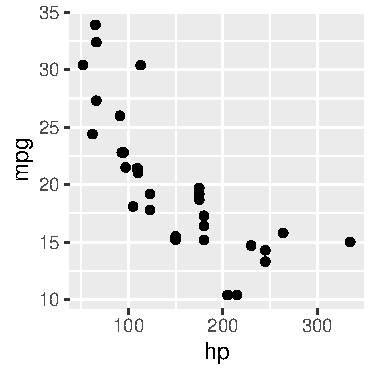
\includegraphics[width=\maxwidth]{figure/unnamed-chunk-4-1} 

}


\end{knitrout}
\end{frame}

\begin{frame}\frametitle{Maximum Likelihood Estimation of OLS Regression}
    \vspace{-1ex}
    $$\texttt{mpg}_i = \beta_0 + \beta_1 \texttt{hp}_i + \varepsilon_i$$ \\
    \vspace{2ex}
    How do we estimate the parameters of this model using ML?
    \vspace{2ex}
    \begin{align*}
        \intertext{For the general regression equation}
        y_i & = \bm{\beta}' \bm{x_i} + \varepsilon_i
        \intertext{with a distributional assumption about the error term}
        \varepsilon_i & \sim \mathcal{N}(0, \sigma^2)
        \intertext{we have a conditional distribution of $y_i$}
        y_i \mid \bm{x}_i & \sim \mathcal{N}(\bm{\beta}' \bm{x_i}, \sigma^2)
    \end{align*}
\end{frame}

\begin{frame}\frametitle{Log-Likelihood Function of OLS Regression}
    If each $y_i$ has a conditional distribution of
    $$y_i \mid \bm{x}_i \sim \mathcal{N}(\bm{\beta}' \bm{x_i}, \sigma^2)$$
    then the (conditional) log-likelihood function is
    $$\ln L(\bm{\beta}, \sigma^2 \mid \bm{y}, \bm{X}) = \sum_{i = 1}^n \ln f(y_i \mid \bm{x_i}, \bm{\beta}, \sigma^2)$$ \\
    \vspace{2ex}
    For our example, we have three parameters to estimate
    $$\bm{\theta} = \left( \beta_0, \beta_1, \sigma^2 \right)$$
    We could take the derivative of $\ln L(\bm{\theta} \mid \bm{y}, \bm{X})$ with respect to each parameter and solve the first-order conditions
    \begin{itemize}
        \item Or we could maximize $\ln L(\bm{\theta} \mid \bm{y}, \bm{X})$ by numerical optimization!
    \end{itemize}
\end{frame}

\begin{frame}\frametitle{Numerical Optimization for MLE}
    We want to find the set of $K$ parameters, $\widehat{\bm{\theta}}$, that maximize the log-likelihood function, $\ln L(\bm{\theta})$
    \begin{enumerate}
        \item Begin with some initial parameter values, $\bm{\theta}^0$
        \item Check if you can ``walk up'' to a higher value
        \item If so, take a step in the right direction to $\bm{\theta}^1$
        \item Repeat steps (2) and (3), stepping from $\bm{\theta}^s$ to $\bm{\theta}^{s + 1}$ until you reach the maximum
    \end{enumerate}
    \vspace{3ex}
    The \texttt{optim()} function in R will perform this numerical optimization for us
    \begin{itemize}
        \item We just have to give the \texttt{optim()} function two things:
        \begin{itemize}
            \item Some initial parameter values, $\bm{\theta}^0$
            \item A function that will take those parameters as an argument and calculate the log-likelihood, $\ln L(\bm{\theta})$
            \item (And sometimes additional information to fine-tune the optimization procedure and output)
        \end{itemize}
    \end{itemize}
\end{frame}

\begin{frame}[fragile]\frametitle{Optimization in R}
\begin{knitrout}\footnotesize
\definecolor{shadecolor}{rgb}{0.969, 0.969, 0.969}\color{fgcolor}\begin{kframe}
\begin{alltt}
\hlcom{## Help file for the optimization function, optim}
\hlopt{?}\hlstd{optim}
\hlcom{## Arguments for optim function}
\hlkwd{optim}\hlstd{(par, fn, gr, ..., method, lower, upper, control, hessian)}
\end{alltt}
\end{kframe}
\end{knitrout}
    \vspace{1ex}
    \texttt{optim()} requires that you create a function, \texttt{fn}, that
    \begin{enumerate}
        \item Takes a set of parameters and other arguments as inputs
        \item Calculates your objective function given those parameters
        \item Returns this value of the objective function
    \end{enumerate}
    \vspace{1ex}
    You also have to give \texttt{optim()} arguments for
    \begin{itemize}
        \item \texttt{par}: starting parameter values
        \item \texttt{\ldots}: dataset and other things needed by your function
        \item \texttt{method}: optimization algorithm
        \begin{itemize}
            \item I recommend \texttt{method = `BFGS'} for our estimation
        \end{itemize}
    \end{itemize}
    \vspace{1ex}
    \texttt{optim()} will find the parameters that minimize the objective function
    \begin{itemize}
        \item To maximize, minimize the negative of the objective function
    \end{itemize}
\end{frame}

\begin{frame}\frametitle{Steps to Calculate the OLS Log-Likelihood}
    The OLS log-likelihood function is
    $$\ln L(\bm{\beta}, \sigma^2 \mid \bm{y}, \bm{X}) = \sum_{i = 1}^n \ln f(y_i \mid \bm{x_i}, \bm{\beta}, \sigma^2)$$
    where the conditional distribution of each $y_i$ is
    $$y_i \mid \bm{x}_i \sim \mathcal{N}(\bm{\beta}' \bm{x_i}, \sigma^2)$$ \\
    \vspace{2ex}
    Steps to calculate the OLS log-likelihood conditional on $\bm{\theta}$
    \begin{enumerate}
        \item Construct matrices $\bm{X}$ and $\bm{y}$ and organize parameters $\bm{\beta}$ and $\sigma^2$
        \item Calculate fitted values of $\bm{y}$, $\widehat{\bm{y}} = \bm{\beta}' \bm{x}_i$, which is the mean of each $y_i$
        \item Calculate the density for each $y_i$, $f(y_i \mid \bm{x}_i, \bm{\theta})$
        \item Calculate the log-likelihood, $\ln L(\bm{\theta} \mid \bm{y}, \bm{X}) = \sum_{i = 1}^n \ln f(y_i \mid \bm{x}_i, \bm{\theta})$
    \end{enumerate}
\end{frame}

\begin{frame}[fragile]\frametitle{Function to Calculate OLS Log-likelihood}
\begin{knitrout}\tiny
\definecolor{shadecolor}{rgb}{0.969, 0.969, 0.969}\color{fgcolor}\begin{kframe}
\begin{alltt}
\hlcom{## Create function to calculate OLS log-likelihood}
\hlstd{ll_ols} \hlkwb{<-} \hlkwa{function}\hlstd{(}\hlkwc{params}\hlstd{,} \hlkwc{data}\hlstd{,} \hlkwc{y_var}\hlstd{,} \hlkwc{x_vars}\hlstd{) \{}
  \hlcom{## Add column of ones for the constant term}
  \hlstd{reg_data} \hlkwb{<-} \hlstd{data} \hlopt
    \hlkwd{mutate}\hlstd{(}\hlkwc{constant} \hlstd{=} \hlnum{1}\hlstd{)}
  \hlcom{## Select data for X and convert to a matrix}
  \hlstd{X} \hlkwb{<-} \hlstd{reg_data} \hlopt
    \hlkwd{select}\hlstd{(}\hlkwd{all_of}\hlstd{(}\hlkwd{c}\hlstd{(}\hlstr{'constant'}\hlstd{, x_vars)))} \hlopt
    \hlkwd{as.matrix}\hlstd{()}
  \hlcom{## Select data for y and convert to a matrix}
  \hlstd{y} \hlkwb{<-} \hlstd{reg_data} \hlopt
    \hlkwd{select}\hlstd{(}\hlkwd{all_of}\hlstd{(y_var))} \hlopt
    \hlkwd{as.matrix}\hlstd{()}
  \hlcom{## Select coefficient parameters}
  \hlstd{beta_hat} \hlkwb{<-} \hlstd{params[}\hlopt{-}\hlkwd{length}\hlstd{(params)]}
  \hlcom{## Select error variance parameters}
  \hlstd{sigma2_hat} \hlkwb{<-} \hlstd{params[}\hlkwd{length}\hlstd{(params)]}
  \hlcom{## Calculate fitted y values}
  \hlstd{y_hat} \hlkwb{<-} \hlstd{X} \hlopt \hlstd{beta_hat}
  \hlcom{## Calculate the pdf values of each outcome}
  \hlstd{y_pdf} \hlkwb{<-} \hlkwd{dnorm}\hlstd{(y,} \hlkwc{mean} \hlstd{= y_hat,} \hlkwc{sd} \hlstd{=} \hlkwd{sqrt}\hlstd{(sigma2_hat))}
  \hlcom{## Calculate the log-likelihood}
  \hlstd{ll} \hlkwb{<-} \hlkwd{sum}\hlstd{(}\hlkwd{log}\hlstd{(y_pdf))}
  \hlcom{## Return the negative of log-likelihood for minimization}
  \hlkwd{return}\hlstd{(}\hlopt{-}\hlstd{ll)}
\hlstd{\}}
\end{alltt}
\end{kframe}
\end{knitrout}
    \vspace{1ex}
    \texttt{optim()} will minimize our objective function
    \begin{itemize}
        \item We will have \texttt{optim()} minimize $-\ln L(\bm{\theta} \mid \bm{y}, \bm{X})$
    \end{itemize}
\end{frame}

\begin{frame}[fragile]\frametitle{Maximize OLS Log-Likelihood}
\begin{knitrout}\footnotesize
\definecolor{shadecolor}{rgb}{0.969, 0.969, 0.969}\color{fgcolor}\begin{kframe}
\begin{alltt}
\hlcom{## Maximize the OLS log-likelihood function}
\hlstd{mle_ols_1} \hlkwb{<-} \hlkwd{optim}\hlstd{(}\hlkwc{par} \hlstd{=} \hlkwd{c}\hlstd{(}\hlnum{0}\hlstd{,} \hlnum{0}\hlstd{,} \hlnum{1}\hlstd{),} \hlkwc{fn} \hlstd{= ll_ols,}
                   \hlkwc{data} \hlstd{= mtcars,} \hlkwc{y_var} \hlstd{=} \hlstr{'mpg'}\hlstd{,} \hlkwc{x_vars} \hlstd{=} \hlstr{'hp'}\hlstd{,}
                   \hlkwc{method} \hlstd{=} \hlstr{'BFGS'}\hlstd{,} \hlkwc{hessian} \hlstd{=} \hlnum{TRUE}\hlstd{)}
\end{alltt}
\end{kframe}
\end{knitrout}
\end{frame}

\begin{frame}[fragile]\frametitle{Optimization Results}
\begin{knitrout}\scriptsize
\definecolor{shadecolor}{rgb}{0.969, 0.969, 0.969}\color{fgcolor}\begin{kframe}
\begin{alltt}
\hlcom{## Show optimization results}
\hlstd{mle_ols_1}
\end{alltt}
\begin{verbatim}
## $par
## [1] 30.09908613 -0.06822967 13.99015277
## 
## $value
## [1] 87.61931
## 
## $counts
## function gradient 
##       84       28 
## 
## $convergence
## [1] 0
## 
## $message
## NULL
## 
## $hessian
##               [,1]         [,2]          [,3]
## [1,]  2.287323e+00 3.355217e+02 -3.520739e-06
## [2,]  3.355217e+02 5.963323e+04  5.199112e-04
## [3,] -3.520739e-06 5.199112e-04  8.174375e-02
\end{verbatim}
\end{kframe}
\end{knitrout}
\end{frame}

\begin{frame}[fragile]\frametitle{Maximum Likelihood Estimator and Standard Errors}
\begin{knitrout}\footnotesize
\definecolor{shadecolor}{rgb}{0.969, 0.969, 0.969}\color{fgcolor}\begin{kframe}
\begin{alltt}
\hlcom{## Show parameter estimates}
\hlstd{mle_ols_1}\hlopt{$}\hlstd{par}
\end{alltt}
\begin{verbatim}
## [1] 30.09908613 -0.06822967 13.99015277
\end{verbatim}
\end{kframe}
\end{knitrout}
    \vspace{1ex}
    $$\widehat{Var}(\widehat{\bm{\theta}}) = \left\{ \left. -\frac{\partial^2 \ln L(\bm{\theta})}{\partial \bm{\theta} \partial \bm{\theta}'} \right\vert_{\bm{\theta} = \widehat{\bm{\theta}}} \right\}^{-1}$$ \\
    \vspace{1ex}
\begin{knitrout}\footnotesize
\definecolor{shadecolor}{rgb}{0.969, 0.969, 0.969}\color{fgcolor}\begin{kframe}
\begin{alltt}
\hlcom{## Calculate MLE standard errors}
\hlstd{mle_ols_1}\hlopt{$}\hlstd{hessian} \hlopt
  \hlkwd{solve}\hlstd{()} \hlopt
  \hlkwd{diag}\hlstd{()} \hlopt
  \hlkwd{sqrt}\hlstd{()}
\end{alltt}
\begin{verbatim}
## [1] 1.58205585 0.00979809 3.49762080
\end{verbatim}
\end{kframe}
\end{knitrout}
\end{frame}

\begin{frame}[fragile]\frametitle{MLE of Another OLS Regression}
    Now use the same optimization function for a different regression
    \begin{itemize}
        \item Regress \texttt{mpg} on \texttt{hp}, \texttt{disp}, \texttt{wt}, \texttt{qsec} from the \texttt{mtcars} dataset
    \end{itemize}
\begin{knitrout}\footnotesize
\definecolor{shadecolor}{rgb}{0.969, 0.969, 0.969}\color{fgcolor}\begin{kframe}
\begin{alltt}
\hlcom{## Maximize the OLS log-likelihood function}
\hlstd{mle_ols_2} \hlkwb{<-} \hlkwd{optim}\hlstd{(}\hlkwc{par} \hlstd{=} \hlkwd{c}\hlstd{(}\hlkwd{rep}\hlstd{(}\hlnum{0}\hlstd{,} \hlnum{5}\hlstd{),} \hlnum{1}\hlstd{),} \hlkwc{fn} \hlstd{= ll_ols,}
                   \hlkwc{data} \hlstd{= mtcars,} \hlkwc{y_var} \hlstd{=} \hlstr{'mpg'}\hlstd{,}
                   \hlkwc{x_vars} \hlstd{=} \hlkwd{c}\hlstd{(}\hlstr{'hp'}\hlstd{,} \hlstr{'disp'}\hlstd{,} \hlstr{'wt'}\hlstd{,} \hlstr{'qsec'}\hlstd{),}
                   \hlkwc{method} \hlstd{=} \hlstr{'BFGS'}\hlstd{,} \hlkwc{hessian} \hlstd{=} \hlnum{TRUE}\hlstd{)}
\hlcom{## Show parameter estimates}
\hlstd{mle_ols_2}\hlopt{$}\hlstd{par}
\end{alltt}
\begin{verbatim}
## [1] 29.171504479 -0.021155823  0.002340875 -4.508394892  0.447863784
## [6]  5.901025047
\end{verbatim}
\begin{alltt}
\hlcom{## Calculate MLE standard errors}
\hlstd{mle_ols_2}\hlopt{$}\hlstd{hessian} \hlopt
  \hlkwd{solve}\hlstd{()} \hlopt
  \hlkwd{diag}\hlstd{()} \hlopt
  \hlkwd{sqrt}\hlstd{()}
\end{alltt}
\begin{verbatim}
## [1] 8.017208039 0.014478340 0.009948106 1.173009722 0.432869462
## [6] 1.500889360
\end{verbatim}
\end{kframe}
\end{knitrout}
\end{frame}

\begin{frame}[fragile]\frametitle{MLE of Another OLS Regression}
    Try a different dataset in our optimization function
    \begin{itemize}
        \item Regress \texttt{Petal.Length} on \texttt{Petal.Width}, \texttt{Sepal.Length}, and \texttt{Sepal.Width} from the \texttt{iris} dataset
    \end{itemize}
\begin{knitrout}\footnotesize
\definecolor{shadecolor}{rgb}{0.969, 0.969, 0.969}\color{fgcolor}\begin{kframe}
\begin{alltt}
\hlcom{## Maximize the OLS log-likelihood function}
\hlstd{mle_ols_3} \hlkwb{<-} \hlkwd{optim}\hlstd{(}\hlkwc{par} \hlstd{=} \hlkwd{c}\hlstd{(}\hlkwd{rep}\hlstd{(}\hlnum{0}\hlstd{,} \hlnum{4}\hlstd{),} \hlnum{1}\hlstd{),} \hlkwc{fn} \hlstd{= ll_ols,}
                   \hlkwc{data} \hlstd{= iris,} \hlkwc{y_var} \hlstd{=} \hlstr{'Petal.Length'}\hlstd{,}
                   \hlkwc{x_vars} \hlstd{=} \hlkwd{c}\hlstd{(}\hlstr{'Petal.Width'}\hlstd{,} \hlstr{'Sepal.Length'}\hlstd{,}
                              \hlstr{'Sepal.Width'}\hlstd{),}
                   \hlkwc{method} \hlstd{=} \hlstr{'BFGS'}\hlstd{,} \hlkwc{hessian} \hlstd{=} \hlnum{TRUE}\hlstd{)}
\hlcom{## Show parameter estimates}
\hlstd{mle_ols_3}\hlopt{$}\hlstd{par}
\end{alltt}
\begin{verbatim}
## [1] -0.26270817  1.44679345  0.72913805 -0.64601245  0.09902641
\end{verbatim}
\begin{alltt}
\hlcom{## Calculate MLE standard errors}
\hlstd{mle_ols_3}\hlopt{$}\hlstd{hessian} \hlopt
  \hlkwd{solve}\hlstd{()} \hlopt
  \hlkwd{diag}\hlstd{()} \hlopt
  \hlkwd{sqrt}\hlstd{()}
\end{alltt}
\begin{verbatim}
## [1] 0.29342388 0.06670595 0.05753860 0.06758029 0.01143187
\end{verbatim}
\end{kframe}
\end{knitrout}
\end{frame}

\end{document}
